\section{Sơ đồ ERD (Entity Relationship Diagram)}
\begin{figure}[H]
    \centering
    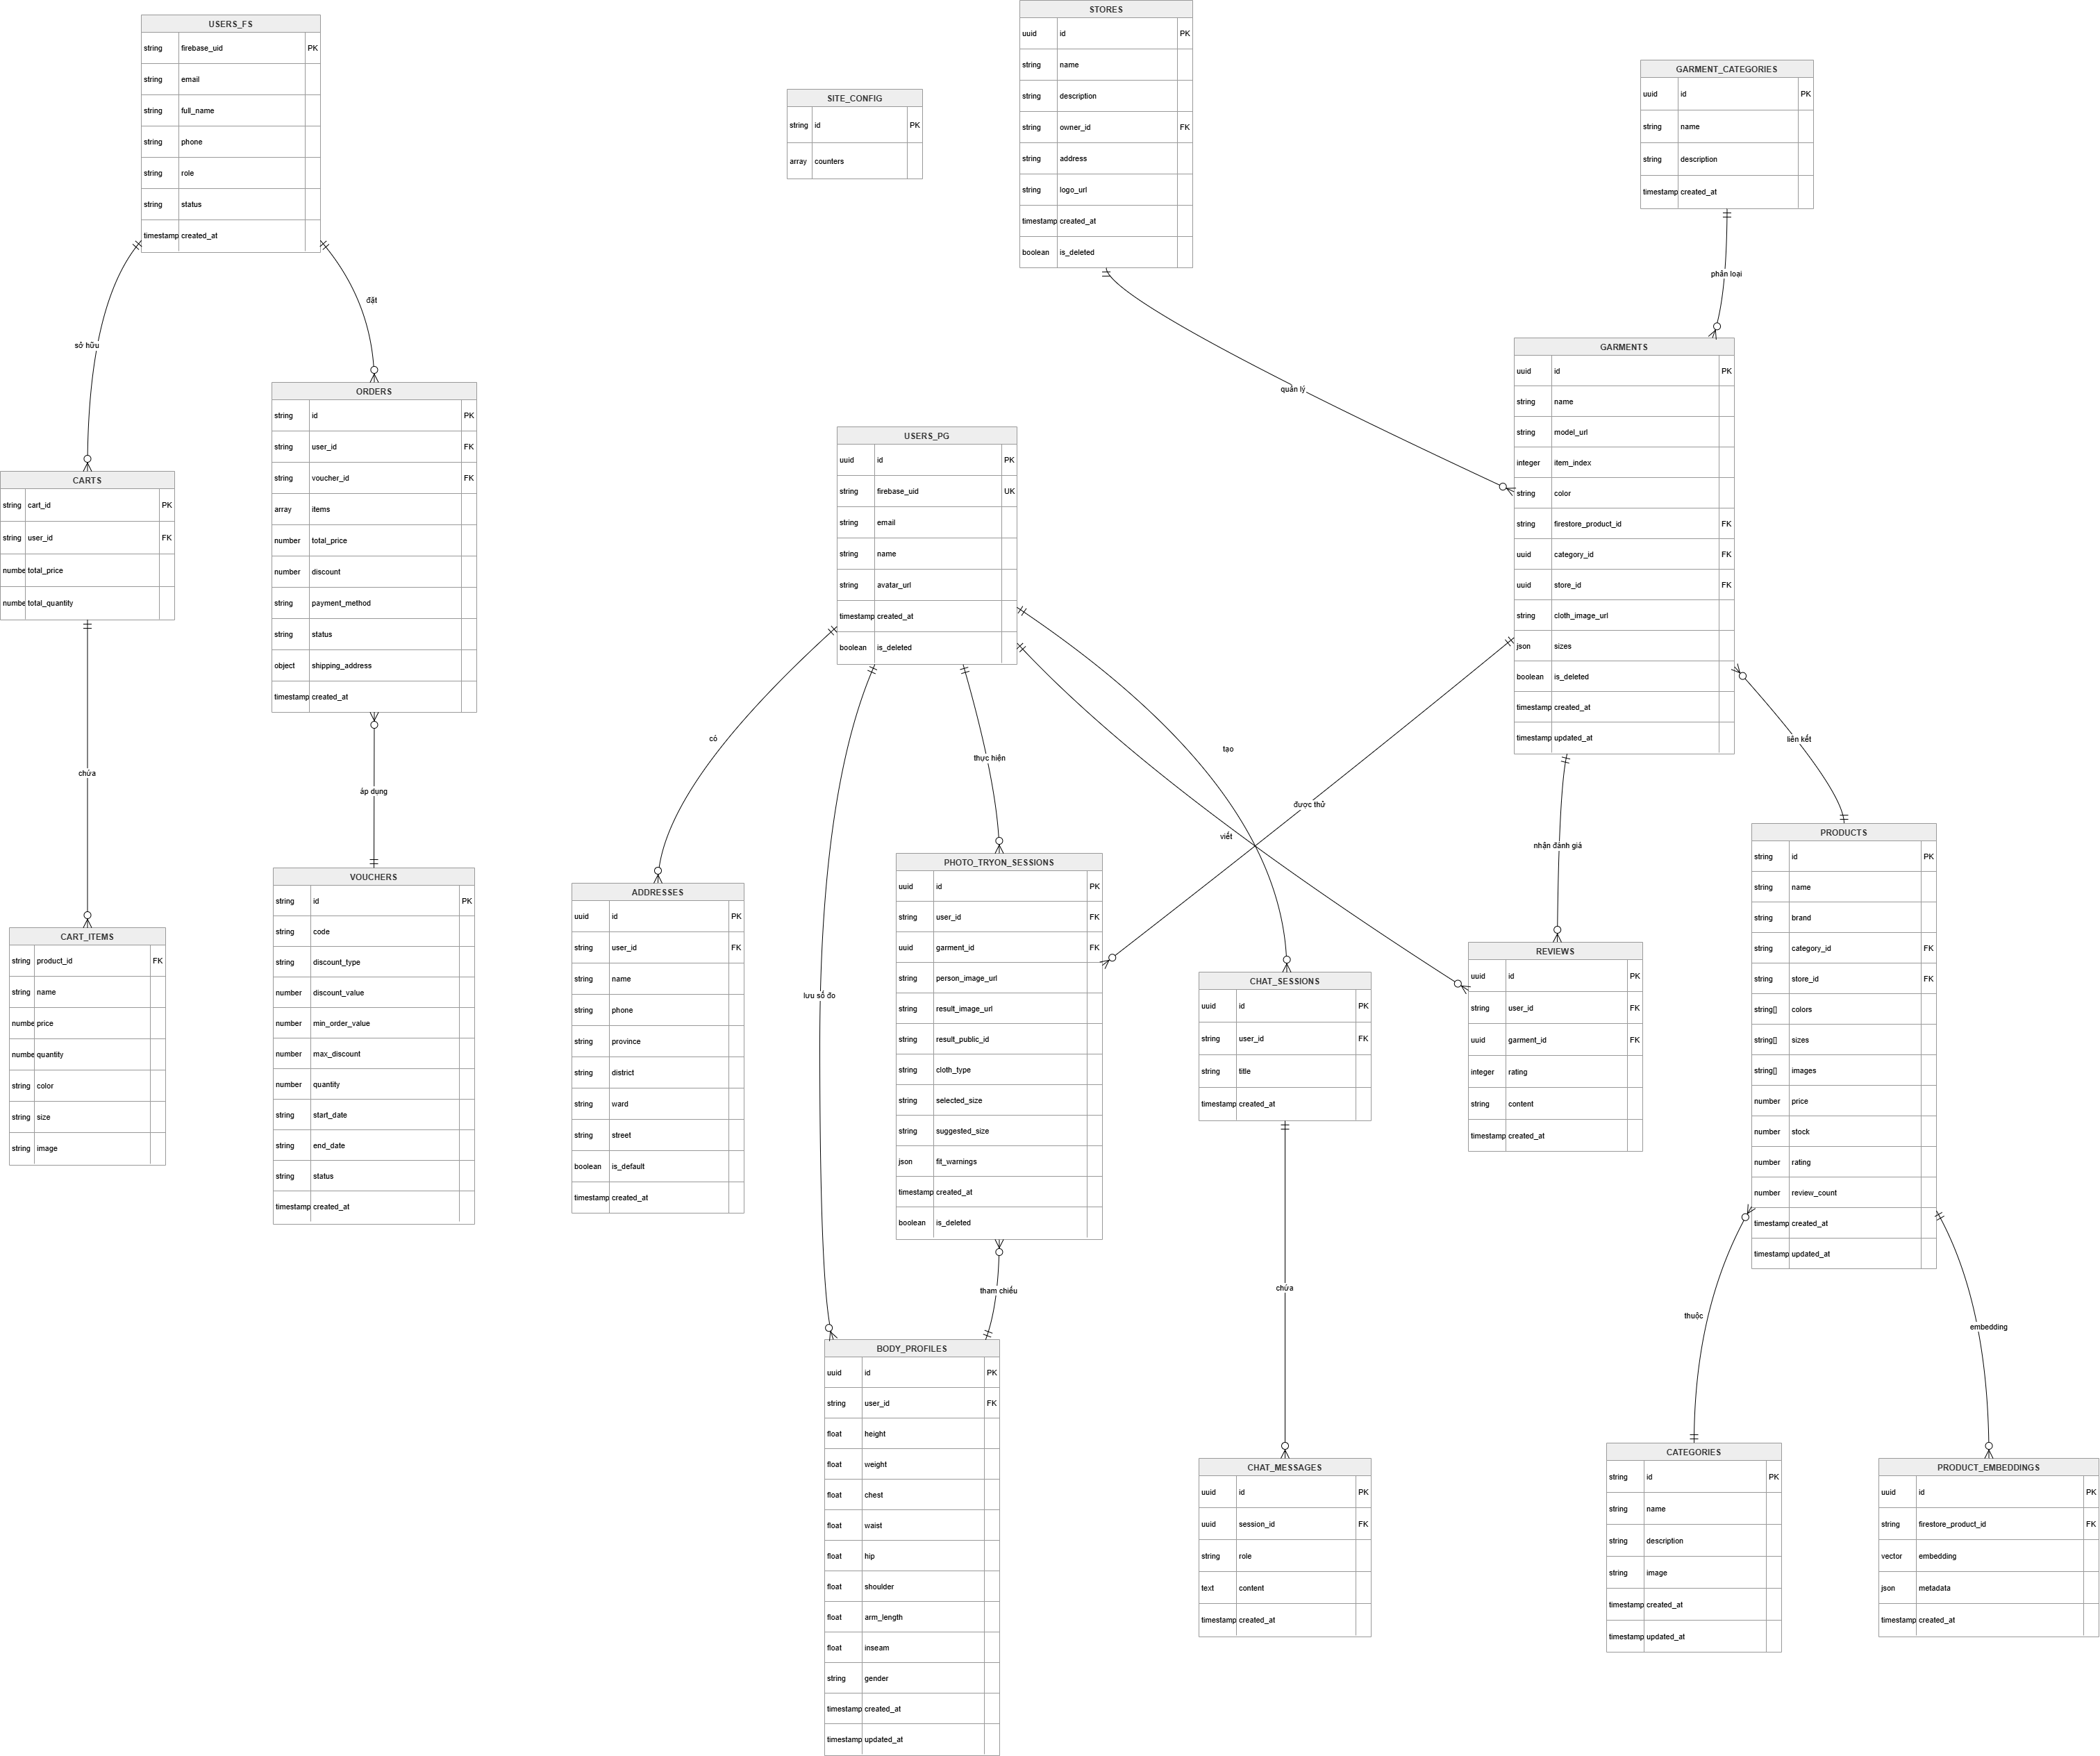
\includegraphics[width=0.9\textwidth]{graphics/main/chapter2/section6/erd2.png}
    \caption{Sơ đồ ERD của hệ thống Virtual Try-On}
    \label{fig:erd_vton}
\end{figure}

\subsection*{Các thực thể}

Cơ sở dữ liệu của hệ thống được thiết kế theo kiến trúc kép gồm Firebase Firestore (NoSQL) và Neon PostgreSQL (quan hệ), với các thực thể chính sau:

\textbf{Firebase Firestore:}
\begin{itemize}[noitemsep]
    \item \textbf{Users\_FS}: Lưu thông tin tài khoản người dùng, phân quyền và trạng thái tài khoản. Xác thực thông qua Firebase Auth (Google Sign-In).
    \item \textbf{Categories}: Lưu danh mục sản phẩm thời trang (Áo, Quần, Túi...) kèm ảnh đại diện Cloudinary.
    \item \textbf{Products}: Lưu thông tin sản phẩm bao gồm tên, thương hiệu, màu sắc, kích cỡ, hình ảnh, giá bán và tồn kho.
    \item \textbf{Carts}: Lưu giỏ hàng của người dùng với tổng số lượng và tổng giá trị.
    \item \textbf{Cart\_Items}: Lưu chi tiết từng sản phẩm trong giỏ hàng gồm màu sắc, size và số lượng.
    \item \textbf{Orders}: Lưu đơn hàng sau thanh toán bao gồm danh sách sản phẩm, địa chỉ giao hàng, phương thức thanh toán và trạng thái đơn.
    \item \textbf{Vouchers}: Lưu mã giảm giá với điều kiện áp dụng, giá trị giảm và thời hạn sử dụng.
    \item \textbf{Site\_Config}: Lưu thông tin giới thiệu cửa hàng (counters, vị trí hiển thị trên bản đồ Leaflet).
\end{itemize}

\textbf{Neon PostgreSQL:}
\begin{itemize}[noitemsep]
    \item \textbf{Users\_PG}: Lưu thông tin người dùng phía PostgreSQL, liên kết với Firebase qua \texttt{firebase\_uid}.
    \item \textbf{Addresses}: Lưu các địa chỉ giao hàng của người dùng, hỗ trợ nhiều địa chỉ với một địa chỉ mặc định.
    \item \textbf{Stores}: Lưu thông tin cửa hàng bao gồm tên, địa chỉ và logo.
    \item \textbf{Garment\_Categories}: Lưu danh mục trang phục dành riêng cho module AR và AI Try-On.
    \item \textbf{Garments}: Lưu thông tin trang phục ảo gồm file GLB (AR Try-On), ảnh flat-lay (FitDiT), \texttt{item\_index} (Snap Carousel) và thông số kỹ thuật từng size.
    \item \textbf{Body\_Profiles}: Lưu số đo cơ thể người dùng (ngực, eo, hông, vai, tay, chân) phục vụ tính năng gợi ý size.
    \item \textbf{Photo\_Tryon\_Sessions}: Lưu lịch sử phiên thử đồ AI gồm ảnh đầu vào, ảnh kết quả FitDiT, size được gợi ý và cảnh báo vùng không vừa.
    \item \textbf{Reviews}: Lưu đánh giá và nhận xét của người dùng đối với từng trang phục.
    \item \textbf{Chat\_Sessions}: Lưu các phiên hội thoại với chatbot tư vấn thời trang.
    \item \textbf{Chat\_Messages}: Lưu nội dung từng tin nhắn trong phiên chat, phân biệt vai trò \texttt{user} và \texttt{assistant}.
    \item \textbf{Product\_Embeddings}: Lưu vector embedding (1536 chiều) của sản phẩm phục vụ tìm kiếm ngữ nghĩa cho chatbot RAG.
\end{itemize}

\subsection*{Mối quan hệ giữa các thực thể}

Người dùng là trung tâm của hệ thống, liên kết với hầu hết các thực thể. Mỗi người dùng có thể sở hữu một giỏ hàng, đặt nhiều đơn hàng, lưu nhiều địa chỉ giao hàng, tạo nhiều phiên chat và thực hiện nhiều phiên thử đồ AI.

Sản phẩm Firestore và Garments PostgreSQL được liên kết thông qua \texttt{firestore\_product\_id}, cho phép một sản phẩm có thể có nhiều phiên bản trang phục ảo tương ứng phục vụ cho AR Try-On và AI Virtual Try-On. Mỗi trang phục thuộc về một cửa hàng và một danh mục, đồng thời chứa thông số kỹ thuật chi tiết từng size phục vụ thuật toán Fit Assessment.

Phiên thử đồ AI liên kết trang phục với người dùng, lưu lại toàn bộ thông tin đầu vào và kết quả sinh ảnh của FitDiT, bao gồm gợi ý size và cảnh báo các vùng không vừa dựa trên số đo cơ thể người dùng.

Chatbot RAG sử dụng bảng \texttt{product\_embeddings} để tìm kiếm ngữ nghĩa qua pgvector, kết hợp với lịch sử hội thoại trong \texttt{chat\_sessions} và \texttt{chat\_messages} để cung cấp tư vấn thời trang cá nhân hóa.